\documentclass{article}

\usepackage[english]{babel}

\usepackage[a4paper,top=2cm,bottom=2cm,left=2cm,right=2cm,marginparwidth=1.75cm]{geometry}
\usepackage{mathtools}
% Useful packages
\usepackage{amsmath}
\usepackage{listings} % for code listing
\usepackage{array}  % for fixed width in table
\usepackage{longtable}  % for table spanning multiple pages
\usepackage{graphicx}
\usepackage[colorlinks=true, allcolors=blue]{hyperref}

% bibliography
\usepackage{biblatex} %Imports biblatex package
\addbibresource{references.bib} %Import the bibliography file

% Utility commands
\newcommand{\fakesection}[1]{%
  % \par \refstepcounter{section}% Increase section counter
  \sectionmark{#1}% Add section mark (header)
  \addcontentsline{toc}{section}{- #1}% Add section to ToC
  % Add more content here, if needed.
}

\newcommand{\literaturereview}[7]{
  \footnotesize #1 &
  \footnotesize #2 &
  \footnotesize #3 &
  \footnotesize #4 &
  \footnotesize #5 &
  \footnotesize #6 &
  \footnotesize #7 \\
 \hline
}


% Contains code for deduplicating same Certifcate, Acknowledgement
\newenvironment{certificatepage}[2]{
\newpage
\begin{center}
    \large \textbf{CERTIFICATE}
\end{center}

% https://tex.stackexchange.com/questions/67571/no-hyphen-for-a-word
\hyphenation{Dissertation}

\large I hereby certify that the work which is being presented in the B.Tech. Dissertation entitled, Shor’s Factorization Algorithm on Quantum Computer in partial fulfillment of the requirements for the award of the Bachelor of Technology in Computer Science and Engineering is an authentic record of my own work carried out during a period from July ,2022 to Nov,2022 under the supervision of Dr. Bhaskar Mondal, Assistant Professor, Computer Science and  Engineering Department. \\

\large The matter presented in this thesis has not been submitted for the award of any other degree elsewhere. \\

\vspace{10ex}
% \hfill \textit{Signature of Candidate} \\

% \hfill Abhay Kumar Chaurasiya \\

% \hfill Roll No. 1906081 \\

\begin{flushright}
\textit{Signature of Candidate} \\

#1 \\

Roll No. #2 \\
\end{flushright}

\text{} \\

This is to certify that the above statement made by the candidate is correct to the best of my knowledge. 

\begin{flushright}
\vspace{10ex}
\textit{Signature of Supervisor} \\

Dr. Bhaskar Mondal  \\

Assistant Professor \\
\end{flushright}

Date:   
}{}


\newenvironment{acknowledgementpage}[1]{
\newpage
\begin{center}
    \large \textbf{ACKNOWLEDGEMENT}
\end{center}

\vspace{2ex}

First of all, I express my gratitude to the Almighty, who blessed me with the zeal and enthusiasm to complete this research work successfully. I am extremely thankful to my supervisors' Dr. Bhaskar Mondal, Assistant Professor, Computer Science and Engineering Department, National Institute of Technology Patna, Patna for their motivation and tireless efforts to help me to get deep knowledge of the research area and for supporting me throughout the life cycle of my B. Tech. dissertation work. Especially, the extensive comments, healthy discussions, and fruitful interactions with the supervisors had a direct impact on the final form and quality of B. Tech. dissertation work. \\

I am also thankful to the Name of The Dr. M. P. Singh, Head of the Computer Science and Engineering Department, for his fruitful guidance through the early years of chaos and confusion. I wish to thank the faculty members and supporting staff of the Computer Science and Engineering Department for their full support and heartiest cooperation. \\

This thesis would not have been possible without the hearty support of my friends. My deepest regards to my Parents for their blessings, affection, and continuous support. Also, Last but not least, I thank GOD, the almighty for giving me the inner willingness, strength, and wisdom to carry out this research work successfully. 

\hfill #1
}{}


\title{\huge Implementation of Shor’s Factorization Algorithm on Quantum Computer}
\author{}

\date{\vspace{-5ex}}

\begin{document}
\maketitle

\begin{center}
    A DISSERTATION \\
    \textit{submitted in fulfillment of the requirements for} \\
    \textit{the award of the degree of}

    \text{\vspace{10ex}} \\
    \text{\vspace{10ex}} \\
    Bachelor of Technology \\
    \text{\vspace{4ex}} \\
    in \\
    \text{\vspace{4ex}} \\
    COMPUTER SCIENCE AND ENGINEERING \\
    \text{\vspace{4ex}} \\
    by \\

    \text{\vspace{4ex}} \\
    \item Abhay Kumar Chaurasiya , 1906081
    \item Aditya Gupta, 1906082
    \item Rabin Gourav Mandal, 1906083

    \text{\vspace{10ex}} \\
    Under the supervision of \\
    Dr Bhaskar Mondal \\
    Assistant Professor \\
\end{center}

\begin{figure}[!htb]
    \centering
    
\includegraphics[width=0.3\textwidth]{images/nitp.png}
\end{figure}

\begin{center}
DEPARTMENT OF COMPUTER ENGINEERING \vspace{3ex} \\
NATIONAL INSTITUTE OF TECHNOLOGY PATNA \vspace{2ex} \\ 
800005, BIHAR (INDIA) \vspace{2ex} \\
December 2022
\end{center}

% Defined in pages/certificate.tex
\fakesection{Certificate}
    \certificatepage{Abhay Kumar Chaurasiya}{1906081}
    \certificatepage{Aditya Gupta}{1906082}
    \certificatepage{Rabin Gaurav Mandal}{1906083}


\fakesection{Acknowledgement}
    \acknowledgementpage{Abhay Kumar Chaurasiya}
    \acknowledgementpage{Aditya Gupta}
    \acknowledgementpage{Rabin Gaurav Mandal}


\newpage
\fakesection{Abstract}
    \begin{center}
        \large \textbf{Abstract}
    \end{center}

    The security of our online transactions rests on the assumption that factoring integers with a thousand or more digits is practically impossible. This assumption was challenged in 1995 when Peter Shor proposed a polynomial-time quantum algorithm for the factoring problem. \\
    
    Quantum computing is a type of computation which operate based on principles from quantum mechanics, such as superposition, and entanglement. \\
    
    Possible uses of quantum computers are thought to
    be capable of solving some computational problems,
    such as integer factorization (which underlies RSA
    encryption), much more quickly than classical
    computers. \\

    An important quantum algorithm for factoring a number N is Shor's algorithm \cite{shor1994polynomial}. Turning the factoring problem into the challenge of determining a function's period is the Shor algorithm's essential strategy. An approach for determining the period of a function is provided, which is based on the fundamental technique and the monotonous of the mode function. \\

    In classical computer, the time complexity for factoring a composite number is $\sqrt{n}$ if we want to find the factor of n. But the Shor's algorithm reduces this time complexity up to O($(log N)^3$ log log N log log logN). This is the biggest motivation to factorize a number using Shor's Algorithm.

\newpage
\tableofcontents

\newpage
\section{Introduction}
A major problem in the field of signal processing is how to construct highly powerful computers. Enhancing the microprocessor's performance is one option. The other technique is developing the computer model and algorithm design through which the problem can be tackled more essentially. The parallel quantum algorithm, a creation of quantum physics and algorithm theory, has seen the most advancement in quantum computing. The fundamental characteristics of the parallel quantum algorithm are based on qubit entanglement, coherence, and quantum superposition.

It is more challenging to factor a fixed large number into two numbers using the traditional approach. That is how public key cryptography works, like RSA, which employs a public key N that is the sum of two very large prime numbers. Shor's algorithm, a typical quantum algorithm created by Shor, can break RSA in a polynomial amount of time. Even more public key cryptosystems have been vulnerable to attack using an extension of Shor's method.

Shor's algorithm, which factors a number N in O($(log N)^3$) time and O(log N) space, is an important quantum algorithm. Turning the factoring problem into the problem of determining a function's period and is a crucial Shor's algorithm trick. The time can be easily achieved by the monotony of the mode function in addition to understanding the character of the mode function. In the meantime, a crucial parameter for period determination is tuned.

It requires $2logN + 2$ quantum bits, where n is the integer to be decomposed.

\section{Problem Definition}

The foundation of modern computation is made up of bits, strings of bits, and the operations we can perform on them.
A bit is a finite field of order 2, frequently abbreviated as F2, and is nothing more than the numbers 0 and 1 multiplied and added modulo 2.
All computation in a conventional computer reduces to representing things as strings of zeroes and ones and then applying Boolean operations to them because the content of a bit is its bit value.
The operation of a quantum computer is not like that.
In quantum computing, one uses unitary maps acting on complex vector spaces rather than Boolean operations acting on binary strings, quantum states rather than bit values, and qubits in place of bits.
A qubit is a quantum bit in physics.

For a physicist, a quantum state is a vector that characterises a physical system, and a qubit is a two-level quantum system.
An n-qubit quantum state is a unit- norm vector in a Hilbert space H = ($C_{2}$ + n), where indicates the tensor product of Hilbert spaces, and a qubit is just the two-dimensional complex Hilbert space $C_{2}$ for a mathematician or computer scientist.
In this report, quantum states and processes will be represented using the Dirac notation. The symbol for a vector in H will be \vert $v_{i}$ $\rangle$, which can be read as "ket v".
We write "bra v" to represent the dual form of $\langle$ $v_{i}$ $\vert$, which is a map from H to C.

In contrast to quantum, we use the term "classical" throughout this report to describe conventional computers and the computations that are performed on them.
The circuits we implement will be collections of horizontal wires, one for each qubit, moving from left to right (research has been done on this also, eg. \cite{zhang2022technique}).
Quantum control wires are the vertical wires that join a qubit and a gate.
A dash between two wires indicates many qubits at once.
Tensor products have occasionally been left out when there is little chance of misinterpretation, as we can write \($\vert$ $\phi_{i}$ ,$\psi_{i}$ $\rangle$\) to denote \($\vert$ $\phi_{i}$ $\rangle$ $\otimes$ $\vert$ $\psi_{i}$ $\rangle$\).

The report will then discuss four quantum algorithms or primitives, beginning with the one that will require the majority of our attention quantum random circuits—and the recent assertion of quantum supremacy. Once the notation has been established, each algorithm or primitive will be discussed in turn. 

In the following section, we discuss the Shor's Algorithm to factor a composite number using IBM's qiskit quantum computer simulator. We have discussed the corresponding theory below.

\section{Period Finding}

The goal of the Shor algorithm is to factorise a huge number N into two small components, $N_{1}$, $N_{2}$. The integers that are smaller than N and include N can easily be seen to form a finite group when multiplied by N. This finite group contains an integer a. In order to accomplish the transformation from the factoring problem to the problem of determining the period of a function, the periodic function is set to the mode function with the integer 'a', so that:

\begin{center}
f(x)=$a^x$$\mod{N}$    
\end{center}

The number 'x' is from 0 to $2^L$ so that $N^2$$\leq$$2^L$$<$$2N^2$ when the number 'a' is from 0 to N-1 and should be combined with N.

The number 'a' may exist a finite order r, which is the smallest positive and even integer such that, because the group of the number 'a' is finite. This relation still holds true for the same integer 'r' if x is set to 0. Thus

\begin{center}

$a^r$$\mod{N}$ \equiv $a^0$$\mod{N}$

$a^r$$\mod{N}$ \equiv 1 $\mod{N} $

\end{center}



Consequently,
\begin{center}

    $a^r$ - 1 = ($a^\frac{r}{2}$+1)($a^\frac{r}{2}$-1) \equiv 0 \mod{N}
    
\end{center}

Here if we put r=0 , that satisfies the equation but 0 is not the answer we want . So we need another non-trivial value of r.So that we can find 
\begin{center}
    $N_{1}$=\gcd($a^\frac{r}{2}$+1,N)

    \newline

    $N_{2}$=\gcd($a^\frac{r}{2}$+1,N)
\end{center}

That satisfies the equation 
\begin{center}
    N=$N_{1}$ $*$ $N_{2}$
\end{center}

\subsection{Algorithm}

Making the factoring problem into the problem of determining a function's period is a crucial Shor's algorithm trick. Another method is to use the Quantum Fourier Transform to determine the function's period. The two methods make up the majority of Shor's algorithm, which may be implemented using the following steps:
 Shor's algorithm for factoring a given integer n can be broken into some simple steps.

\begin{enumerate}
    \item
    Determine if the number n is a prime, a even number, or an integer power of a prime number. If it is we will not use Shor's algorithm. There are efficient classical methods for determining if a integer n belongs to one of the above groups, and providing factors for it if it is. This step would be performed on a classical computer.

    \item
    Pick a integer q that is the power of 2 such that $n^2$ $\leq$ $2^q$ $<$ 2$n^2$. This step would be done on a classical computer.

    \item
    Pick a random integer x that is co-prime to n. When two numbers are co-prime it means that their greatest common divisor is 1. There are efficient classical methods for picking such an x. This step would be done on a classical computer.

    \item
    Create a quantum register and partition it into two parts, register 1 and register 2. Thus the state of our quantum computer can be given by: \vert reg1, reg2$ \rangle$. Register 1 must have enough qubits to represent integers as large as q - 1. Register 2 must have enough qubits to represent integers as large as n - 1. The calculations for how many qubits are needed would be done on a classical computer.

    \item
    Load register 1 with an equally weighted superposition of all integers from 0 to q - 1. Load register 2 with all zeros. This operation would be performed by our quantum computer. The total state of the quantum memory register at this point is:

    \begin{center}
    $\displaystyle {\frac{{1}}{{\sqrt{q}}}}$$\displaystyle \sum_{{a = 0}}^{{q - 1}}$ \vert a, 0$\displaystyle \rangle$
    \end{center}

    \item
    Now apply the transformation xa mod n to for each number stored in register 1 and store the result in register 2. Due to quantum parallelism this will take only one step, as the quantum computer will only calculate x \vert a$\scriptstyle \rangle$ mod n, where \vert a$ \rangle$ is the superposition of states created in step 5. This step is performed on the quantum computer. The state of the quantum memory register at this point is:

    \begin{center}
    $\displaystyle {\frac{{1}}{{\sqrt{q}}}}$$\displaystyle \sum_{{a = 0}}^{{q - 1}}$ \vert a, xa \mod{n}$\displaystyle \rangle$
    \end{center}

    \item
    Measure the second register, and observe some value k. This has the side effect of collapsing register one into a equal superposition of each value a between 0 and q - 1 such that

    \begin{center}
    % TODO
    xa mod n = k
    \end{center}

    This operation is performed by the quantum computer. The state of the quantum memory register after this step is:

    \begin{center}
    $\displaystyle {\frac{{1}}{{\sqrt{\vert\vert A\vert\vert}}}}$$\displaystyle \sum_{{a'=a'\in A}}^{}$ \vert a', k$\displaystyle \rangle$
    \end{center}

    Where A is the set of a's such that xa mod n = k, and $||$A$||$ is the number of elements in that set.

    \item
    Now compute the discrete Fourier transform on register one. The discrete Fourier transform when applied to a state \vert a$ \rangle$ changes it in the following manner:

    \begin{center}
        \vert a$\displaystyle \rangle$ = $\displaystyle {\frac{{1}}{{\sqrt{q}}}}$$\displaystyle \sum_{{c=0}}^{{q-1}}$ \vert c $\displaystyle \rangle$*$\exp(\frac{2\pi i a c}{q})$
    \end{center}

    This step is performed by the quantum computer in one step through quantum parallelism. After the discrete Fourier transform our register is in the state:

    \begin{center}
    
        $\displaystyle {\frac{{1}}{{\sqrt{\vert\vert A\vert\vert}}}}$$\displaystyle \sum_{{a'\in A}}^{}$$\displaystyle {\frac{{1}}{{\sqrt{q}}}}$$\displaystyle \sum_{{c=0}}^{{q-1}}$\vert c,k$\displaystyle \rangle$*$\exp(${(2$\pi$ i a$'$ c)}/{q}$)$
    
    \end{center}

    \item
    Measure the state of register one, call this value m, this integer m has a very high probability of being a multiple of q/r, where r is the desired period. This step is performed by the quantum computer.

    \item
    Take the value m, and on a classical computer do some post processing which calculates r based on knowledge of m and q. In particular:

        m has a high probability of being = $ \lambda$*(q/r) where $ \lambda$ is an integer
        If we perform floating point division of m/q, and then calculate the best rational approximation to m/q whose denominator is less than or equal to q
        We take this denominator to be a candidate for r.
        If our candidate r is odd we either double it if doing so leads to a value less than q

    There are efficient ways to do this post processing on a classical computer.

    \item
    % TODO
    Once you have attained r, a factor of n can be determined by taking gcd($x^\frac{r}{2}$ + 1, n) and gcd($x^\frac{r}{2}$ - 1, n). If you have found a factor of n, then stop, if not go to step 4. This final step is done on a classical computer.
\end{enumerate}

Step 11 contains a provision for what to do if Shor's algorithm failed to produce factors of n. There are a few reasons why Shor's algorithm can fail, for example the discrete Fourier transform could be measured to be 0 in step 9, making the post processing in step 10 impossible. The algorithm will sometimes find factors of 1 and n, which is not useful either. For these reasons step 11 must be able to jump back to step 4 to start over.

\section{Finding Period Using Quantum Computation}

For finding the period for used in shor's algorithm, we use Quantum Phase Estimation, which internally uses Quantum Fourier Transformation. The two are explained in the below subsections. 

\subsection{Quantum Fourier Transformation}

The Fourier transform occurs in many different versions throughout classical computing, in areas ranging from signal processing to data compression to complexity theory. The quantum Fourier transform (QFT) is the quantum implementation of the discrete Fourier transform over the amplitudes of a wavefunction. It is part of many quantum algorithms, most notably Shor's factoring algorithm and quantum phase estimation. The discrete Fourier transform acts on a vector \((x_0, ..., x_{N-1})\) and maps it to the vector \((y_0, ..., y_{N-1})\) according to the formula

\[y_k = \frac{1}{\sqrt{N}}\sum_{j=0}^{N-1}x_j\omega_N^{jk}\]

where \(\omega_N^{jk} = e^{2\pi i \frac{jk}{N}}\).

Similarly, the quantum Fourier transform acts on a quantum state \(\vert X\rangle = \sum_{j=0}^{N-1} x_j \vert j \rangle\) and maps it to the quantum state \(\vert Y\rangle = \sum_{k=0}^{N-1} y_k \vert k \rangle\) according to the formula

\[y_k = \frac{1}{\sqrt{N}}\sum_{j=0}^{N-1}x_j\omega_N^{jk}\]

with \(\omega_N^{jk}\) defined as above. Note that only the amplitudes
of the state were affected by this transformation.

This can also be expressed as the map:

\[\vert j \rangle \mapsto \frac{1}{\sqrt{N}}\sum_{k=0}^{N-1}\omega_N^{jk} \vert k \rangle\]

Or the unitary matrix:

\[ U_{QFT} = \frac{1}{\sqrt{N}} \sum_{j=0}^{N-1} \sum_{k=0}^{N-1} \omega_N^{jk} \vert k \rangle \langle j \vert\]

\hypertarget{intuition}{%
\subsubsection{\texorpdfstring{Intuition}{}}\label{intuition}}

The quantum Fourier transform (QFT) transforms between two bases, the
computational (Z) basis, and the Fourier basis. The H-gate is the
single-qubit QFT, and it transforms between the Z-basis states
\(|0\rangle\) and \(|1\rangle\) to the X-basis states \(|{+}\rangle\)
and \(|{-}\rangle\). In the same way, all multi-qubit states in the
computational basis have corresponding states in the Fourier basis. The
QFT is simply the function that transforms between these bases.

\[
|\text{State in Computational Basis}\rangle \quad \xrightarrow[]{\text{QFT}} \quad |\text{State in Fourier Basis}\rangle
\]

\[
\text{QFT}|x\rangle = |\widetilde{x}\rangle
\]




In the computational basis, we store numbers in binary using the states
\(|0\rangle\) and \(|1\rangle\).

Note the frequency with which the different qubits change; the leftmost
qubit flips with every increment in the number, the next with every 2
increments, the third with every 4 increments, and so on.

The number we want to store dictates the angle at which each qubit is
rotated around the Z-axis. In the state \(|\widetilde{0}\rangle\), all
qubits are in the state \(|{+}\rangle\). As seen in the example above,
to encode the state \(|\widetilde{5}\rangle\) on 4 qubits, we rotated
the leftmost qubit by \(\tfrac{5}{2^n} = \tfrac{5}{16}\) full turns
(\(\tfrac{5}{16}\times 2\pi\) radians). The next qubit is turned double
this (\(\tfrac{10}{16}\times 2\pi\) radians, or \(10/16\) full turns),
this angle is then doubled for the qubit after, and so on.

Again, note the frequency with which each qubit changes. The leftmost
qubit (\texttt{qubit\ 0}) in this case has the lowest frequency, and the
rightmost the highest.


So what does the quantum Fourier transform look like for larger \(N\)?
Let's derive a transformation for \(N=2^n\), \(QFT_N\) acting on the
state \(\vert x \rangle = \vert x_1\ldots x_n \rangle\) where \(x_1\) is
the most significant bit. This maths is here for those that find it
useful, if you struggle with it then don't worry; as long as you
understand the intuition in section 2 then you can continue straight to
the next section.

\[
\begin{aligned}
QFT_N\vert x \rangle & = \frac{1}{\sqrt{N}} \sum_{y=0}^{N-1}\omega_N^{xy} \vert y \rangle 
\\
& = \frac{1}{\sqrt{N}} \sum_{y=0}^{N-1} e^{2 \pi i xy / 2^n} \vert y \rangle ~\text{since}\: \omega_N^{xy} = e^{2\pi i \frac{xy}{N}} \:\text{and}\: N = 2^n 
\\
& = \frac{1}{\sqrt{N}} \sum_{y=0}^{N-1} e^{2 \pi i \left(\sum_{k=1}^n y_k/2^k\right) x} \vert y_1 \ldots y_n \rangle \: y = y_1\ldots y_n, y/2^n = \sum_{k=1}^n y_k/2^k 
\\
& = \frac{1}{\sqrt{N}} \sum_{y=0}^{N-1} \prod_{k=1}^n e^{2 \pi i x y_k/2^k } \vert y_1 \ldots y_n \rangle 
\\
& = \frac{1}{\sqrt{N}} \bigotimes_{k=1}^n  \left(\vert0\rangle + e^{2 \pi i x /2^k } \vert1\rangle \right) 
\sum_{y=0}^{N-1} = \sum_{y_1=0}^{1}\sum_{y_2=0}^{1}\ldots\sum_{y_n=0}^{1} 
\\
& = \frac{1}{\sqrt{N}}
\left(\vert0\rangle + e^{\frac{2\pi i}{2}x} \vert1\rangle\right) 
\otimes
\left(\vert0\rangle + e^{\frac{2\pi i}{2^2}x} \vert1\rangle\right) 
\otimes  
\ldots
\otimes
\left(\vert0\rangle + e^{\frac{2\pi i}{2^{n-1}}x} \vert1\rangle\right) 
\otimes
\left(\vert0\rangle + e^{\frac{2\pi i}{2^n}x} \vert1\rangle\right) 
\end{aligned}
\]

\hypertarget{the-circuit-that-implements-the-qft}{%
\subsubsection{\texorpdfstring{The Circuit that Implements the QFT
}{The Circuit that Implements the QFT }}\label{the-circuit-that-implements-the-qft}}

The circuit that implements QFT makes use of two gates. The first one is
a single-qubit Hadamard gate, \(H\), that you already know.You have
already seen that the action of \(H\) on the single-qubit state
\(\vert x_k\rangle\) is

\[H\vert x_k \rangle = \frac{1}{\sqrt{2}}\left(\vert0\rangle + \exp\left(\frac{2\pi i}{2}x_k\right)\vert1\rangle\right)\]

The second is a two-qubit controlled rotation \(CROT_k\) given in
block-diagonal form as

\[CROT_k = \left[\begin{matrix}
I&0\\
0&UROT_k\\
\end{matrix}\right]\]

where

\[UROT_k = \left[\begin{matrix}
1&0\\
0&\exp\left(\frac{2\pi i}{2^k}\right)\\
\end{matrix}\right]\]

The action of \(CROT_k\) on a two-qubit state \(\vert x_l x_j\rangle\)
where the first qubit is the control and the second is the target is
given by

\[CROT_k\vert 0x_j\rangle = \vert 0x_j\rangle\]

and

\[CROT_k\vert 1x_j\rangle = \exp\left( \frac{2\pi i}{2^k}x_j \right)\vert 1x_j\rangle\]

Given these two gates, a circuit that implements an n-qubit QFT is shown below.

\begin{figure}[!htb]
\centering
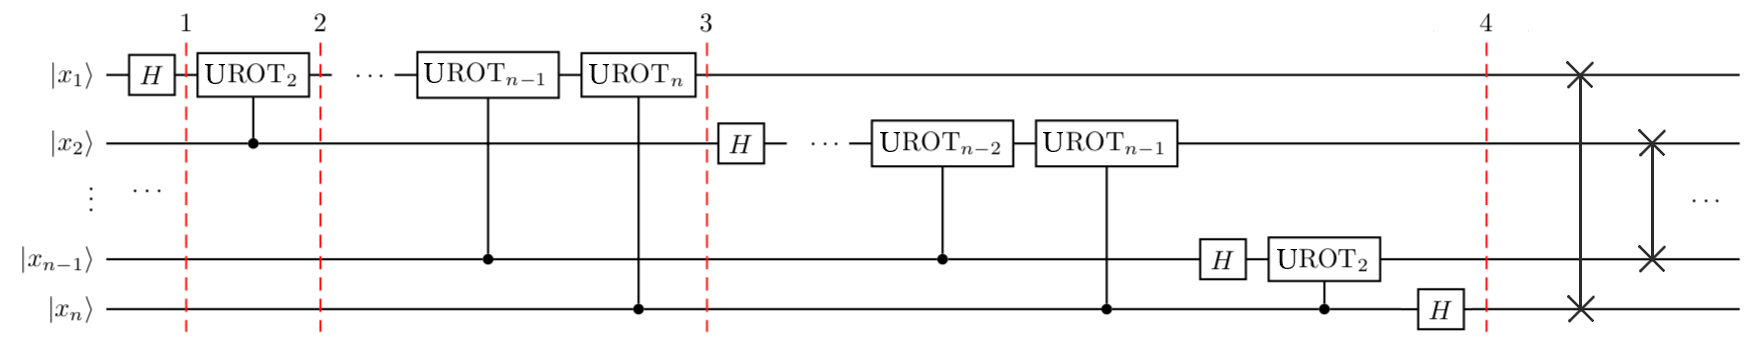
\includegraphics[width=1\textwidth]{images/qft.png}
\caption{QFT Circuit}
\end{figure}

The circuit operates as follows. We start with an n-qubit input state
\(\vert x_1x_2\ldots x_n\rangle\).

After the first Hadamard gate on qubit 1, the state is transformed from
the input state to

\[
H_1\vert x_1x_2\ldots x_n\rangle = 
\frac{1}{\sqrt{2}}
\left[\vert0\rangle + \exp\left(\frac{2\pi i}{2}x_1\right)\vert1\rangle\right]
\otimes
\vert x_2x_3\ldots x_n\rangle
\]

After the \(UROT_2\) gate on qubit 1 controlled by qubit 2, the state is
transformed to

\[
\frac{1}{\sqrt{2}}
\left[\vert0\rangle + \exp\left(\frac{2\pi i}{2^2}x_2 + \frac{2\pi i}{2}x_1\right)\vert1\rangle\right]
\otimes
\vert x_2x_3\ldots x_n\rangle
\]

After the application of the last \(UROT_n\) gate on qubit 1 controlled
by qubit \(n\), the state becomes

\[
\frac{1}{\sqrt{2}}
\left[\vert0\rangle + 
\exp\left(
\frac{2\pi i}{2^n}x_n + 
\frac{2\pi i}{2^{n-1}}x_{n-1} + 
\ldots + 
\frac{2\pi i}{2^2}x_2 + 
\frac{2\pi i}{2}x_1
\right)
\vert1\rangle\right]
\otimes
\vert x_2x_3\ldots x_n\rangle
\]

Noting that

\[
x = 2^{n-1}x_1 + 2^{n-2}x_2 + \ldots + 2^1x_{n-1} + 2^0x_n
\]

we can write the above state as

\[
\frac{1}{\sqrt{2}}
\left[\vert0\rangle + 
\exp\left(
\frac{2\pi i}{2^n}x 
\right)
\vert1\rangle\right]
\otimes
\vert x_2x_3\ldots x_n\rangle
\]

After the application of a similar sequence of gates for qubits
\(2\ldots n\), we find the final state to be:

\[
\frac{1}{\sqrt{2}}
\left[\vert0\rangle + 
\exp\left(
\frac{2\pi i}{2^n}x 
\right)
\vert1\rangle\right]
\otimes
\frac{1}{\sqrt{2}}
\left[\vert0\rangle + 
\exp\left(
\frac{2\pi i}{2^{n-1}}x 
\right)
\vert1\rangle\right]
\otimes
\ldots
\otimes
\frac{1}{\sqrt{2}}
\left[\vert0\rangle + 
\exp\left(
\frac{2\pi i}{2^{1}}x 
\right)
\vert1\rangle\right]
\]

Which is exactly the QFT of the input state as derived above with the
caveat that the order of the qubits is reversed in the output state.

\hypertarget{example-1-1-qubit-qft}{%
\subsubsection{\texorpdfstring{Example: 1-qubit QFT
}{}}\label{example-1-1-qubit-qft}}

Consider how the QFT operator as defined above acts on a single qubit
state
\(\vert\psi\rangle = \alpha \vert 0 \rangle + \beta \vert 1 \rangle\).
In this case, \(x_0 = \alpha\), \(x_1 = \beta\), and \(N = 2\). Then,

\[y_0 = \frac{1}{\sqrt{2}}\left(    \alpha \exp\left(2\pi i\frac{0\times0}{2}\right) + \beta \exp\left(2\pi i\frac{1\times0}{2}\right)      \right) = \frac{1}{\sqrt{2}}\left(\alpha + \beta\right)\]

and

\[y_1 = \frac{1}{\sqrt{2}}\left(    \alpha \exp\left(2\pi i\frac{0\times1}{2}\right) + \beta \exp\left(2\pi i\frac{1\times1}{2}\right)      \right) = \frac{1}{\sqrt{2}}\left(\alpha - \beta\right)\]

such that the final result is the state

\[U_{QFT}\vert\psi\rangle = \frac{1}{\sqrt{2}}(\alpha + \beta) \vert 0 \rangle + \frac{1}{\sqrt{2}}(\alpha - \beta)  \vert 1 \rangle\]

This operation is exactly the result of applying the Hadamard operator
(\(H\)) on the qubit:

\[H = \frac{1}{\sqrt{2}}\begin{bmatrix} 1 & 1 \\ 1 & -1 \end{bmatrix}\]

If we apply the \(H\) operator to the state
\(\vert\psi\rangle = \alpha \vert 0 \rangle + \beta \vert 1 \rangle\),
we obtain the new state:

\[\frac{1}{\sqrt{2}}(\alpha + \beta) \vert 0 \rangle + \frac{1}{\sqrt{2}}(\alpha - \beta)  \vert 1 \rangle 
\equiv \tilde{\alpha}\vert 0 \rangle + \tilde{\beta}\vert 1 \rangle\]

Notice how the Hadamard gate performs the discrete Fourier transform for
\(N = 2\) on the amplitudes of the state.

\subsection{Quantum Phase Estimation}

Quantum phase estimation is one of the most important subroutines in
quantum computation. It serves as a central building block for many
quantum algorithms. The objective of the algorithm is the following:

Given a unitary operator \(U\), the algorithm estimates \(\theta\) in
\(U\vert\psi \rangle =e^{\boldsymbol{2\pi i} \theta }|\psi \rangle\).
Here \(|\psi\rangle\) is an eigenvector and
\(e^{\boldsymbol{2\pi i}\theta}\) is the corresponding eigenvalue. Since
U is unitary, all of its eigenvalues have a norm of 1.

\hypertarget{intuition}{%

\subsubsection{\texorpdfstring{Intuition
}{}}\label{intuition}}

The phase of \(U\) (in the Fourier basis) is written to the \(t\) qubits in the counting register by the quantum phase estimation technique using phase kickback.
Then, we convert this from the Fourier basis to the computational basis, which we can measure, using the inverse QFT.

In the Fourier basis, the topmost qubit completes one full revolution while counting between \(0\) and \(2^t\). 

We spin this qubit by \(\tfrac{x}{2^t}\) around the z-axis to count to a number, x, between (0, 2t). We rotate by \(\tfrac{2x}{2^t}\) for the following qubit and by \(\tfrac{4x}{2^t}\) for the following qubit.


When a qubit is used to control the \(U\)-gate, the kickback effect causes the qubit to turn proportionally to the phase \(e^{2i\pi\theta}\).
The phase theta can be encoded as a number between \(0\) and \(2^t\) in the Fourier basis by using successive "\(CU\)-gates" to repeat this rotation an appropriate number of times.

Then we simply use \(QFT^\dagger\) to convert this into the
computational basis.

\hypertarget{mathematical-foundation}{%
\subsubsection{\texorpdfstring{Mathematical Foundation
}{}}\label{mathematical-foundation}}

As mentioned above, this circuit estimates the phase of a unitary
operator \(U\). It estimates \(\theta\) in
\(U\vert\psi \rangle =e^{\boldsymbol{2\pi i} \theta }|\psi \rangle\),
where \(|\psi\rangle\) is an eigenvector and
\(e^{\boldsymbol{2\pi i}\theta}\) is the corresponding eigenvalue. The
circuit operates in the following steps:

\begin{enumerate}
\def\labelenumi{\roman{enumi}.}
\tightlist
\item
  \textbf{Setup}: \(\vert\psi\rangle\) is in one set of qubit registers.
  An additional set of \(n\) qubits form the counting register on which
  we will store the value \(2^n\theta\):
\end{enumerate}

\[ |\psi_0\rangle = \lvert 0 \rangle^{\otimes n} \lvert \psi \rangle\]

\begin{enumerate}
\def\labelenumi{\roman{enumi}.}
\setcounter{enumi}{1}
\tightlist
\item
  \textbf{Superposition}: Apply a \(n\)-bit Hadamard gate operation (efficient methods in eg. \cite{barrera2003new})
  \(H^{\otimes n}\) on the counting register:
\end{enumerate}

\[ |\psi_1\rangle = {\frac {1}{2^{\frac {n}{2}}}}\left(|0\rangle +|1\rangle \right)^{\otimes n} \lvert \psi \rangle\]

\begin{enumerate}
\def\labelenumi{\roman{enumi}.}
\setcounter{enumi}{2}
\tightlist
\item
  \textbf{Controlled Unitary Operations}: We need to introduce the
  controlled unitary \(CU\) that applies the unitary operator \(U\) on
  the target register only if its corresponding control bit is
  \(|1\rangle\). Since \(U\) is a unitary operator with eigenvector
  \(|\psi\rangle\) such that
  \(U|\psi \rangle =e^{\boldsymbol{2\pi i} \theta }|\psi \rangle\), this
  means:
\end{enumerate}

\[U^{2^{j}}|\psi \rangle =U^{2^{j}-1}U|\psi \rangle =U^{2^{j}-1}e^{2\pi i\theta }|\psi \rangle =\cdots =e^{2\pi i2^{j}\theta }|\psi \rangle\]

Applying all the \(n\) controlled operations \(CU^{2^j}\) with
\(0\leq j\leq n-1\), and using the relation
\(|0\rangle \otimes |\psi \rangle +|1\rangle \otimes e^{2\pi i\theta }|\psi \rangle =\left(|0\rangle +e^{2\pi i\theta }|1\rangle \right)\otimes |\psi \rangle\):

\begin{aligned}
|\psi_{2}\rangle & =\frac {1}{2^{\frac {n}{2}}} \left(|0\rangle+{e^{\boldsymbol{2\pi i} \theta 2^{n-1}}}|1\rangle \right) \otimes \cdots \otimes \left(|0\rangle+{e^{\boldsymbol{2\pi i} \theta 2^{1}}}\vert1\rangle \right) \otimes \left(|0\rangle+{e^{\boldsymbol{2\pi i} \theta 2^{0}}}\vert1\rangle \right) \otimes |\psi\rangle\\\\
& = \frac{1}{2^{\frac {n}{2}}}\sum _{k=0}^{2^{n}-1}e^{\boldsymbol{2\pi i} \theta k}|k\rangle \otimes \vert\psi\rangle
\end{aligned}

where \(k\) denotes the integer representation of n-bit binary numbers.

\begin{enumerate}
\def\labelenumi{\roman{enumi}.}
\setcounter{enumi}{3}
\tightlist
\item
  \textbf{Inverse Fourier Transform}: Notice that the above expression
  is exactly the result of applying a quantum Fourier transform as we
  derived in the notebook on
  Quantum Fourier Transform and its Qiskit Implementation. Recall that QFT maps
  an n-qubit input state \(\vert x\rangle\) into an output as
\end{enumerate}

\[
QFT\vert x \rangle = \frac{1}{2^\frac{n}{2}}
\left(\vert0\rangle + e^{\frac{2\pi i}{2}x} \vert1\rangle\right) 
\otimes
\left(\vert0\rangle + e^{\frac{2\pi i}{2^2}x} \vert1\rangle\right) 
\otimes  
\ldots
\otimes
\left(\vert0\rangle + e^{\frac{2\pi i}{2^{n-1}}x} \vert1\rangle\right) 
\otimes
\left(\vert0\rangle + e^{\frac{2\pi i}{2^n}x} \vert1\rangle\right) 
\]

Replacing \(x\) by \(2^n\theta\) in the above expression gives exactly
the expression derived in step 2 above. Therefore, to recover the state
\(\vert2^n\theta\rangle\), apply an inverse Fourier transform on the
auxiliary register. Doing so, we find

\[
\vert\psi_3\rangle = \frac {1}{2^{\frac {n}{2}}}\sum _{k=0}^{2^{n}-1}e^{\boldsymbol{2\pi i} \theta k}|k\rangle \otimes | \psi \rangle \xrightarrow{\mathcal{QFT}_n^{-1}} \frac {1}{2^n}\sum _{x=0}^{2^{n}-1}\sum _{k=0}^{2^{n}-1} e^{-\frac{2\pi i k}{2^n}(x - 2^n \theta)} |x\rangle \otimes |\psi\rangle
\]

\begin{enumerate}
\def\labelenumi{\alph{enumi}.}
\setcounter{enumi}{21}
\tightlist
\item
  \textbf{Measurement}: The above expression peaks near
  \(x = 2^n\theta\). For the case when \(2^n\theta\) is an integer,
  measuring in the computational basis gives the phase in the auxiliary
  register with high probability:
\end{enumerate}

\[ |\psi_4\rangle = | 2^n \theta \rangle \otimes | \psi \rangle\]

For the case when \(2^n\theta\) is not an integer, it can be shown that
the above expression still peaks near \(x = 2^n\theta\) with probability
better than \(4/\pi^2 \approx 40\%\).

\newpage


\section{Literature Review}

\begin{table}[h!]
\centering
% \begin{longtable}{| p{.20\textwidth} | p{.80\textwidth} |} 
\begin{tabular}{| p{10em} | p{4em} | p{6.5em} | p{5em} | p{4em} | p{4em} | p{6em} |} 
% \begin{longtable}{| p{10em} | p{4em} | p{6.5em} | p{5em} | p{4em} | p{4em} | p{6em} |} 
 \hline
  Author \& Year & Algo Name & Implementation method & Advancement & Limitation & List of Test & Threat to \\ [0.5ex]
 \hline\hline
  \literaturereview{J. V. Burke; A. S. Lewis; M. L. Overton, 2008 \cite{burke2008speed}}
      {Shor’ Algorithm}
      {Iterative Shor’s}
      {Proving linear convergence in 2-dimensional case}
      {Available number of qubits}
      {Exact Line Search \& Convex quadratic}
      {Factorisation problem based Cryptographic methods}

  \literaturereview{Shah Muhammad Hamdi, Syed Tauhid Zuhori, Firoz Mahmud, Biprodip Pal, 2014 \cite{hamdi2014compare}}
      {General Number Field Sieve}
      {General Number Field Sieve}
      {Most efficient algorithms, cannot factor integers which are 1000 decimal digits}
      {Calculation speed of classical computers}
      {Comparsion with Shor’s Algorithm}
      {RSA}

  \literaturereview{Kunal Dey, Sumit Kumar Debnath, Pantelimon Stănică, Vikas Srivastava; 2022 \cite{dey2022post}}
      {Isogeny based signcryption scheme}
      {SimS \cite{fouotsa2021sims} and SeaSign}
      {Post-Quantum Cryptographic Algorithm}
      {Not practical currently}
      {IND − CCA and EUF − CMA security checks}
      {-}

  \literaturereview{P. W. Shor; 1994 \cite{shor1994polynomial}}
      {Shor' Algorithm}
      {Integer Factorization}
      {Polynomial-time algorithms for prime factorization and discrete logarithms on a quantum computer}
      {Difficult Implementation for bigger numbers}
      {-}
      {RSA}

  \literaturereview{S. Aaronson and A. Arkhipov; 2011 \cite{aaronson2011computational}}
      {Bason Sampling}
      {PH infinite or approx. counting}
      {The computational complexity of linear optics}
      {Difficult to verify}
      {PH infinite counting}
      {Breaks assumption of PH infinite}

  \literaturereview{D. Shepherd and M. J. Bremner; 2009 \cite{shepherd2009temporally}}
      {IQP}
      {Quantum Computation}
      {Temporally unstructured quantum computation}
      {Difficult to verify}
      {QUATH \cite{aaronson2016complexity}, P-hard \cite{bouland2018quantum}}
      {-}

  \literaturereview{Pierre A. Deymier, Keith Runge, M. Arif Hasan; 2022 \cite{runge2022demonstration}}
      {Deutsch–Jozsa algorithm}
      {Deutsch-like algorithm}
      {Two quantum-like algorithms which exploit classical entanglement (i.e., nonseparability) of elastic waves}
      {-}
      {-}

  \literaturereview{A. Amaricci, L. Crippa, A. Scazzola b, F. Petocchid, G. Mazzae; 2022 \cite{amaricci2022edipack}}
      {EDIpack}
      {Look-up method}
      {Exact diagonalization package to solve generic quantum impurity problems}
      {Exponential growth of the Hilbert space is the bottleneck of ED calculations}
      {Lanczos or P-Arpack algorithm}
      {-}

  \literaturereview{Song, Hui-Chao and Liu, Xiao-Nan and Jiang, Duo and An, Jiale; 2022 \cite{song2022grover}}
      {Efficient Grover}
      {IBM Q quantum cloud platform}
      {Influence of different noises on the circuit
under different iterations was explored}
      {Noise in quantum circuits}
      {No Noise Experiment, Experiment with Noise}
      {-}

% \caption{Literature review of various papers}
% \label{table:1}
% \end{longtable}
\end{tabular}
\caption{Literature review of various papers}
\label{table:1}
\end{table}

\newpage
\section{Results and Analysis}

Shor's solution was to use quantum phase estimation on the
unitary operator:

\[ U|y\rangle \equiv |ay \bmod N \rangle \]

To see how this is helpful, let's work out what an eigenstate of U might
look like. If we started in the state \(|1\rangle\), we can see that
each successive application of U will multiply the state of our register
by \(a \pmod N\), and after \(r\) applications we will arrive at the
state \(|1\rangle\) again. For example with \(a = 3\) and \(N = 35\):

\[\begin{aligned}
U|1\rangle &= |3\rangle & \\
U^2|1\rangle &= |9\rangle \\
U^3|1\rangle &= |27\rangle \\
& \vdots \\
U^{(r-1)}|1\rangle &= |12\rangle \\
U^r|1\rangle &= |1\rangle 
\end{aligned}\] So a superposition of the states in this cycle
(\(|u_0\rangle\)) would be an eigenstate of \(U\):

\[|u_0\rangle = \tfrac{1}{\sqrt{r}}\sum_{k=0}^{r-1}{|a^k \bmod N\rangle} \]

Example with \(a = 3\) and \(N=35\):

\[\begin{aligned}
|u_0\rangle &= \tfrac{1}{\sqrt{12}}(|1\rangle + |3\rangle + |9\rangle \dots + |4\rangle + |12\rangle) \\[10pt]
U|u_0\rangle &= \tfrac{1}{\sqrt{12}}(U|1\rangle + U|3\rangle + U|9\rangle \dots + U|4\rangle + U|12\rangle) \\[10pt]
 &= \tfrac{1}{\sqrt{12}}(|3\rangle + |9\rangle + |27\rangle \dots + |12\rangle + |1\rangle) \\[10pt]
 &= |u_0\rangle
\end{aligned}\]

This eigenstate has an eigenvalue of 1, which isn't very interesting. A
more interesting eigenstate could be one in which the phase is different
for each of these computational basis states. Specifically, let's look
at the case in which the phase of the \(k\)th state is proportional to
\(k\):

\[\begin{aligned}
|u_1\rangle &= \tfrac{1}{\sqrt{r}}\sum_{k=0}^{r-1}{e^{-\tfrac{2\pi i k}{r}}|a^k \bmod N\rangle}\\[10pt]
U|u_1\rangle &= e^{\tfrac{2\pi i}{r}}|u_1\rangle 
\end{aligned}
\]

Example with \(a = 3\) and \(N=35\)

\[\begin{aligned}
|u_1\rangle &= \tfrac{1}{\sqrt{12}}(|1\rangle + e^{-\tfrac{2\pi i}{12}}|3\rangle + e^{-\tfrac{4\pi i}{12}}|9\rangle \dots + e^{-\tfrac{20\pi i}{12}}|4\rangle + e^{-\tfrac{22\pi i}{12}}|12\rangle) \\[10pt]
U|u_1\rangle &= \tfrac{1}{\sqrt{12}}(|3\rangle + e^{-\tfrac{2\pi i}{12}}|9\rangle + e^{-\tfrac{4\pi i}{12}}|27\rangle \dots + e^{-\tfrac{20\pi i}{12}}|12\rangle + e^{-\tfrac{22\pi i}{12}}|1\rangle) \\[10pt]
U|u_1\rangle &= e^{\tfrac{2\pi i}{12}}\cdot\tfrac{1}{\sqrt{12}}(e^{\tfrac{-2\pi i}{12}}|3\rangle + e^{-\tfrac{4\pi i}{12}}|9\rangle + e^{-\tfrac{6\pi i}{12}}|27\rangle \dots + e^{-\tfrac{22\pi i}{12}}|12\rangle + e^{-\tfrac{24\pi i}{12}}|1\rangle) \\[10pt]
U|u_1\rangle &= e^{\tfrac{2\pi i}{12}}|u_1\rangle
\end{aligned}\]

(We can see \(r = 12\) appears in the denominator of the phase.)

This is a particularly interesting eigenvalue as it contains \(r\). In
fact, \(r\) has to be included to make sure the phase differences
between the \(r\) computational basis states are equal. This is not the
only eigenstate with this behaviour; to generalise this further, we can
multiply an integer, \(s\), to this phase difference, which will show up
in our eigenvalue:

\[\begin{aligned}
|u_s\rangle &= \tfrac{1}{\sqrt{r}}\sum_{k=0}^{r-1}{e^{-\tfrac{2\pi i s k}{r}}|a^k \bmod N\rangle}\\[10pt]
U|u_s\rangle &= e^{\tfrac{2\pi i s}{r}}|u_s\rangle 
\end{aligned}
\]

Since the computational basis state \(|1\rangle\) is a superposition of
these eigenstates, which means if we do QPE on \(U\) using the state
\(|1\rangle\), we will measure a phase:

\[\phi = \frac{s}{r}\]

Where \(s\) is a random integer between \(0\) and \(r-1\). We finally
use the continued fractions algorithm on \(\phi\) to find \(r\). The circuit diagram
looks like this (note that this diagram uses Qiskit's qubit ordering
convention):

Using these, we demonstrated the Shor's algorithm using Qiskit's simulators. For
this demonstration we will provide the circuits for \(U\) without
explanation, but in section 4 we will discuss how circuits for
\(U^{2^j}\) can be constructed efficiently.

\section{Conclusion \& Future Scope}

We factored a composite number. If we increase the number of qubits used by quantum computers then the value of n in RSA can be factorized and this will be a big threat to our cryptosystem.
We ran it on IBM’s qiskit platform, on real quantum computers, as well as simulators.
We also used AWS platform to utilize AWS’s quantum computers provided by the AWS braket.

Shor’s algorithms (including its enhanced versions) depend over number of qubits for factoring large composite numbers.
Current maximum is about 433 by IBM, this can be increased in future.
Post-Quantum cryptographic algorithms \cite{borges2020comparison} \cite{nguyen2022novel} can be used instead of algorithms that depend on factorisation problems.

\printbibliography %Prints bibliography

\end{document}
